\section{Mode 0 Operation}

\begin{figure}[h!]
  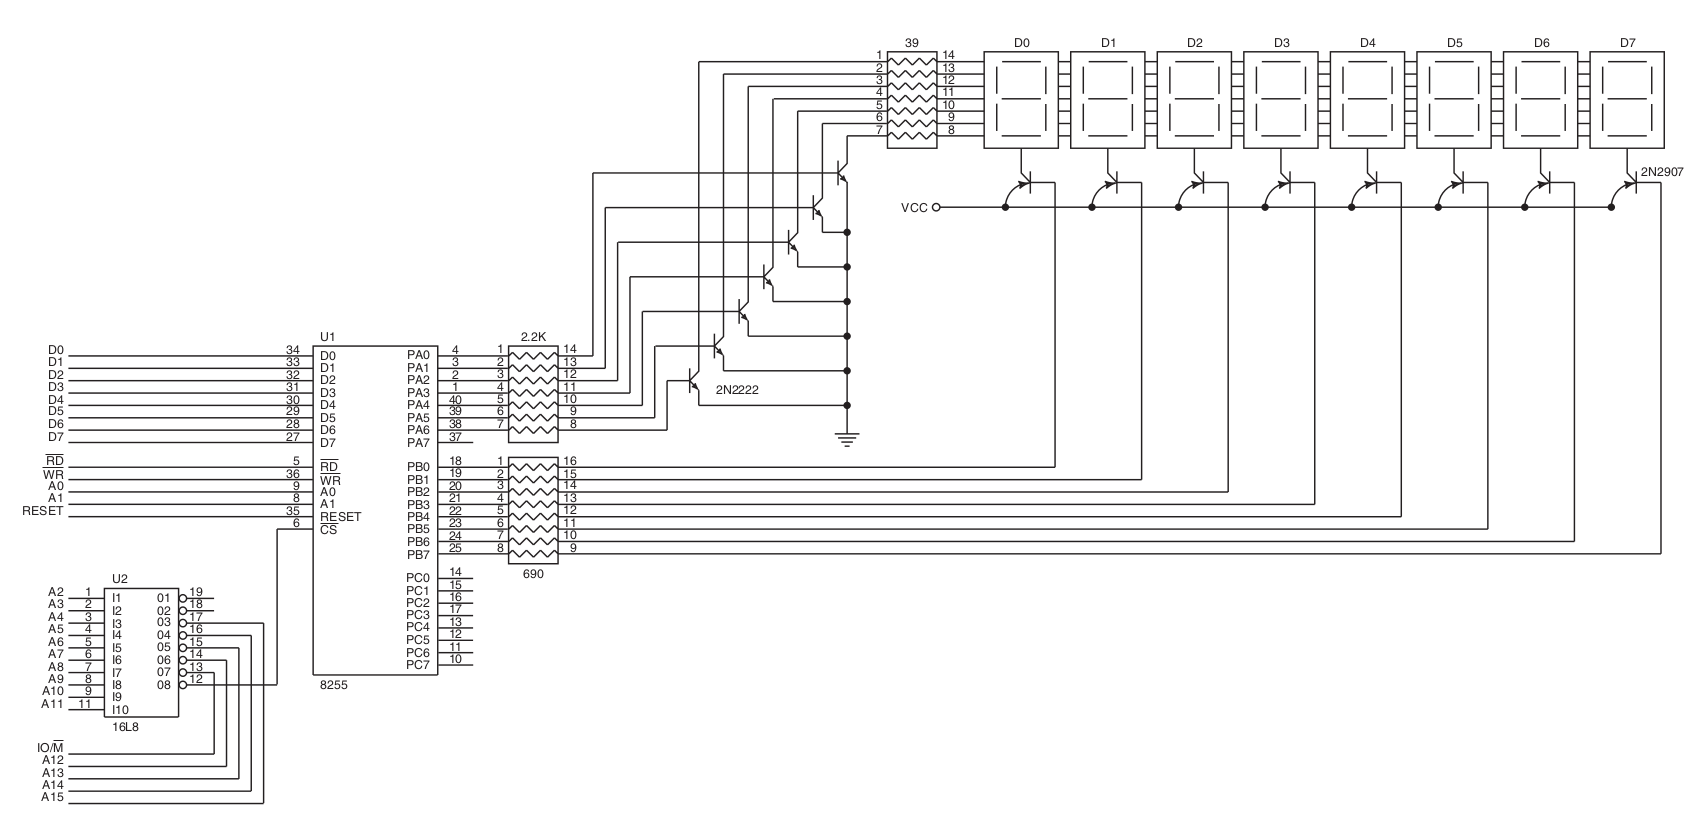
\includegraphics[width = 1.2\textwidth]{./figures/Mode_0_op.png}
  \caption{An 8-digit LED display interfaced to the 8088 microprocessor through an 82C55 PIA.}
\end{figure}

PAL Logic:
\begin{enumerate}
  \item $\overline{CS} = \overline{A15} \cdot \overline{A14} \cdot \overline{A13} \cdot \overline{A12} \cdot \overline{A11} \cdot \overline{A10} \cdot \overline{A9} \cdot \overline{A8} \cdot \overline{A7} \cdot \overline{A6} \cdot \overline{A5} \cdot \overline{A4} \cdot \overline{A3} \cdot \overline{A2} \cdot \overline{IO}$
  \item 82C55 is interfaced to an 808 microprocessor through a PAL 16L8 so that it functions at I/O port numbers 0700H - 0703H
  \item Resistors are chosen to limit segment current
  \item Different assembly code (\textbf{SELF-STUDY})
\end{enumerate}

\subsection{Mode 0 Operation: Keyboard Matrix interface}

\begin{figure}[h!]
  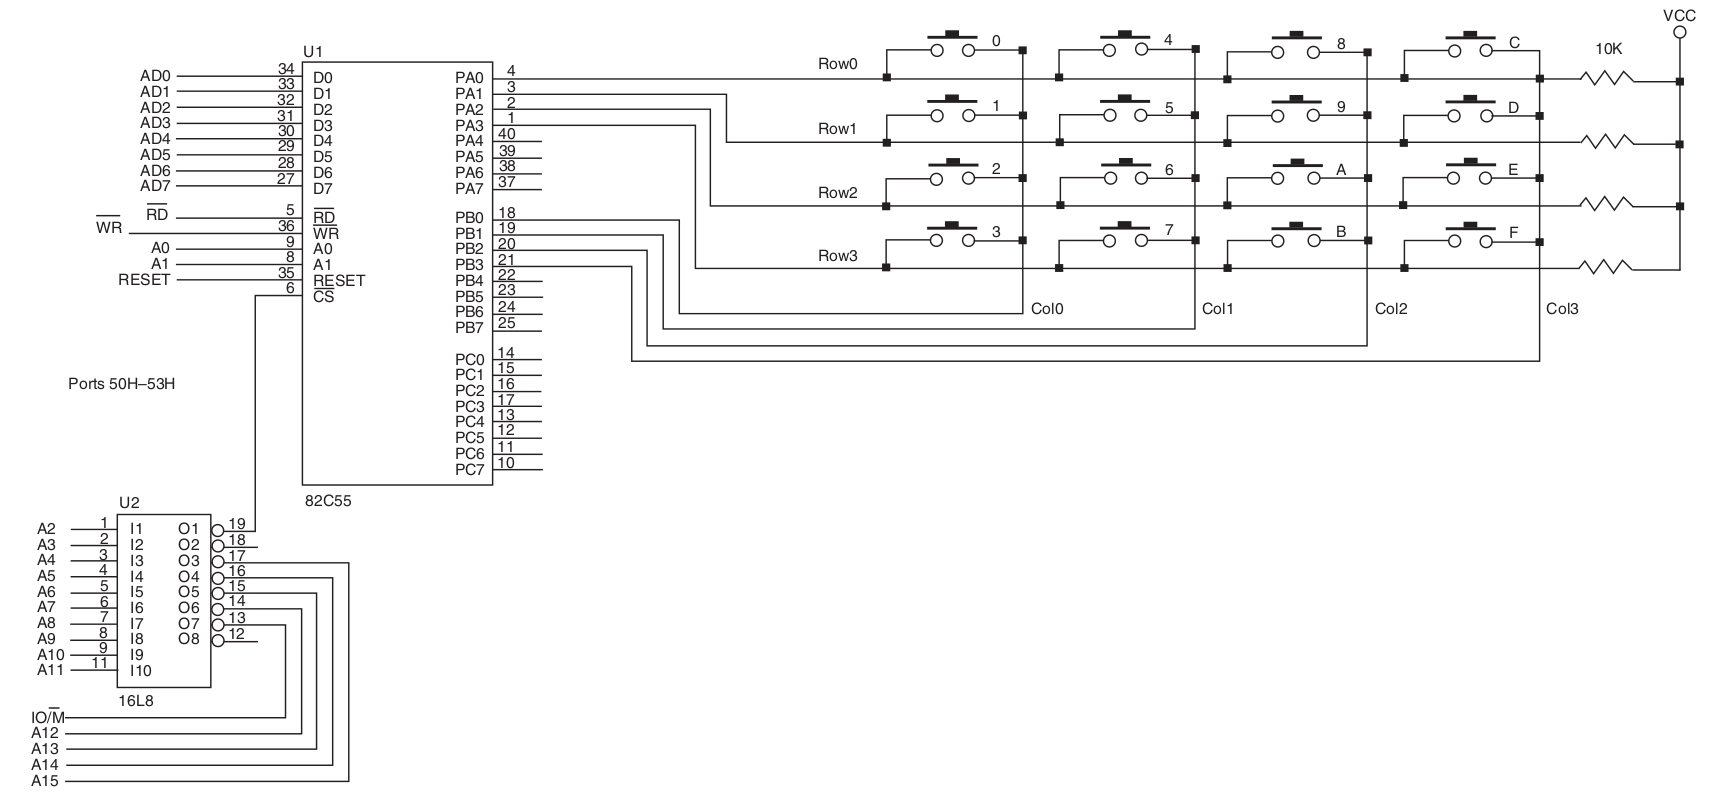
\includegraphics[width = 1.2\textwidth]{./figures/Mode_0_key.png}
  \caption{A 4 x 4 keyboard matrix connected to an 8088 microprocessor through the 82C55 PIA.}
\end{figure}

\begin{itemize}
  \item \textbf{Port A}: Input
  \item \textbf{Port B}: Output
  \item One O is put in Port B (Ex:0111); Column with 0 gets selected. Any key pressing in that column gives 0 to corresponding row
  \item Have logic for debouncing (Flow Chart)

\end{itemize}

\begin{figure}[h!]
  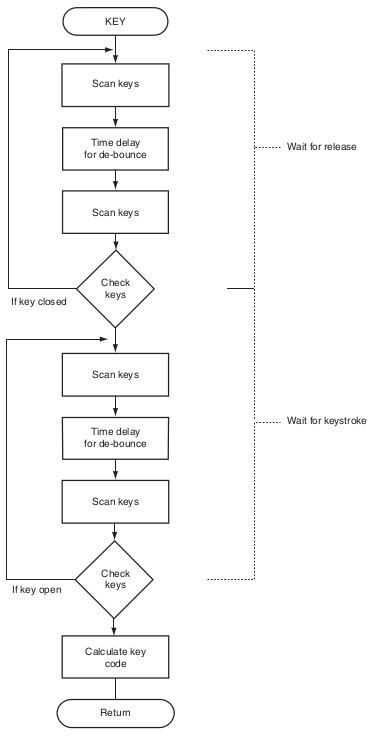
\includegraphics[width = 0.7\textwidth]{./figures/Debounce.png}
  \caption{The flowchart of a keyboard-scanning procedure.}
\end{figure}
\newpage
\section{Mode 1: Strobed Input}
Allows external data to be stored into the port until the microprocessor is ready to receive it.
\begin{figure}[h!]
  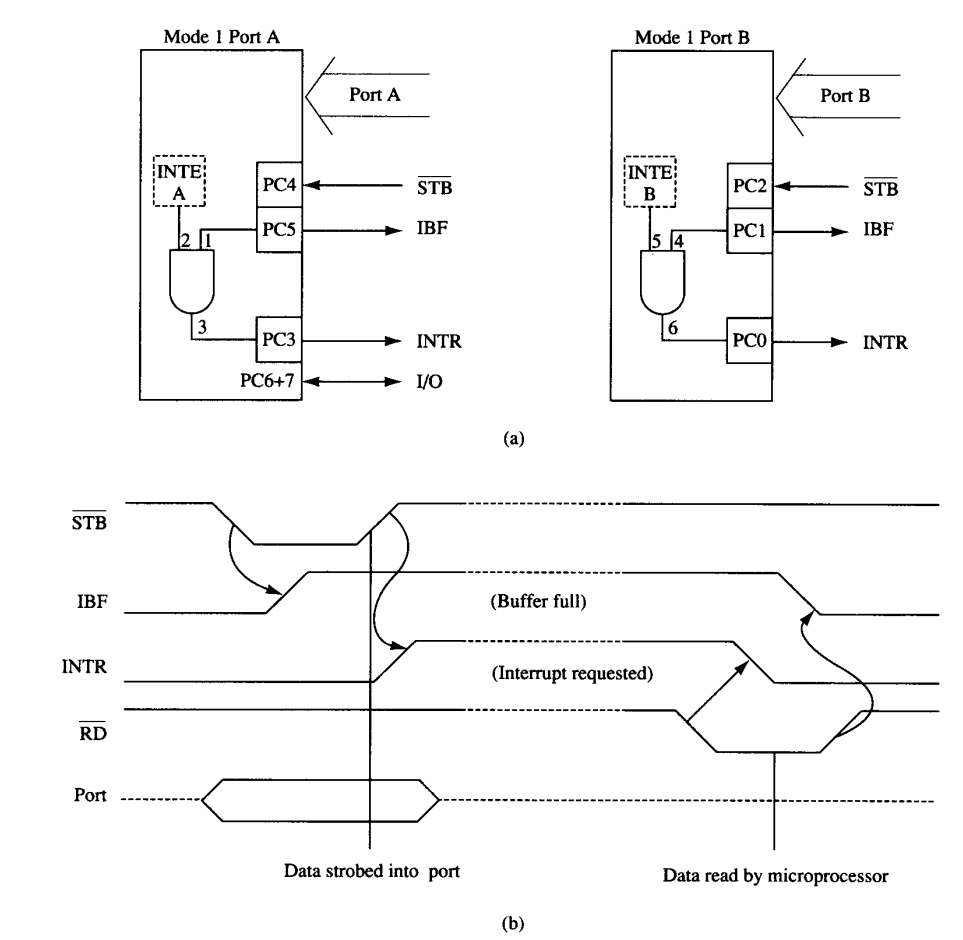
\includegraphics[width = 1.2\textwidth]{./figures/Mode_1.png}
  \caption{Strobed input operation (mode 1) of the 82C55. (a) Internal structure and (b) timing diagram.}
\end{figure}

\begin{description}
  \item[$\overline{STB}$] The \textbf{strobe} input loads data into the port latch, which holds the information until it is input to the microprocessor via the IN instruction.
  \item[IBF] \textbf{Input buffer full} is an output indicating that the input latch contains information.
  \item[INTR] \textbf{Interrupt request} is an output that requests an interrupt. The INTR pin becomes a logic 1 when the $\overline{STB}$ input returns to a logic 1, and is cleared when the data are input from the port by the microprocessor.
  \item[INTE] The \textbf{Interrupt enable} signal is neither an input nor an output; it is an internal bit programmed via the port PC 4 (port A) or PC 2 (port B) bit position.
  \item[PC 6,7] The port C pins 7 and 6 are general-purpose I/O pins that are available for any purpose.

\end{description}
\begin{figure}[h!]
  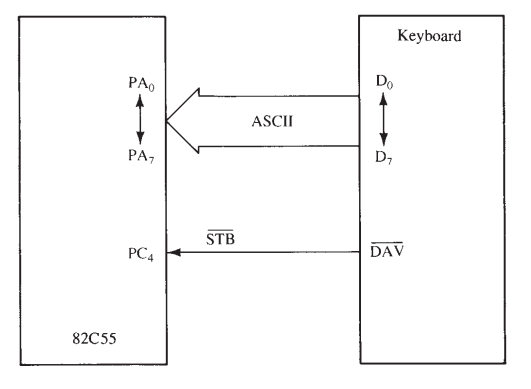
\includegraphics[width = 0.8\textwidth]{./figures/Strobed.png}
  \caption{Using the 82C55 for strobed input operation of a keyboard.}
\end{figure}
\begin{itemize}
  \item The keyboard encoder debounces keyswitches, and gives $\overline{STB}$ if a key is pressed.
  \item $\overline{DAV}$ (Data available) is activated for $1.0 \mu s$ each time a key is typed (Gives $\overline{STB}$)
\end{itemize}


\section{Mode 1: Strobed Output}
\begin{figure}[h!]
  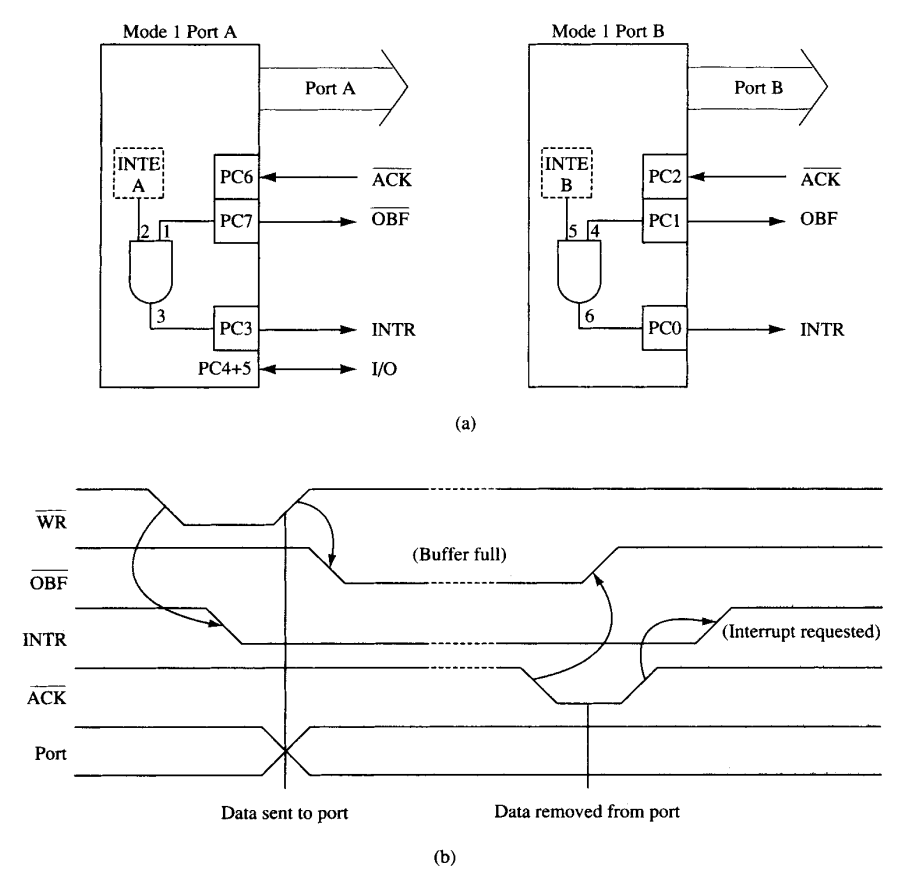
\includegraphics[width = 1.2\textwidth]{./figures/Strobed_Output.png}
  \caption{Strobed output operation (mode 1) of the 82C55. (a) Internal structure and (b) timing diagram.}
\end{figure}

\begin{description}
  \item[$\overline{OBF}$] Output buffer full is an output that goes low whenever data are output (OUT) to the port A or port B latch. This signal is set to a logic 1 whenever the ACK pulse returns from the external device.
  \item[$\overline{ACK}$] The acknowledge signal causes the OBF pin to return to a logic 1 level. The ACK signal is a response from an external device, indicating that it has received the data from the 82C55 port.
  \item[INTR] Interrupt request is a signal that often interrupts the microprocessor when the external device receives the data via the ACK signal. This pin is qualified by the internal INTE (interrupt enable) bit.
  \item[INTE] Interrupt enable is neither an input nor an output; it is an internal bit programmed to enable or disable the INTR pin. The INTE A bit is programmed using the PC 6 bit and INTE B is programmed using the PC 2 bit.
  \item[$PC_4 , PC_5$] Port C pins PC 4 and PC 5 are general-purpose I/O pins. The bit set and reset command is used to set or reset these two pins.
\end{description}

\subsection{Strobed Output: Printer}

\begin{figure}[h!]
  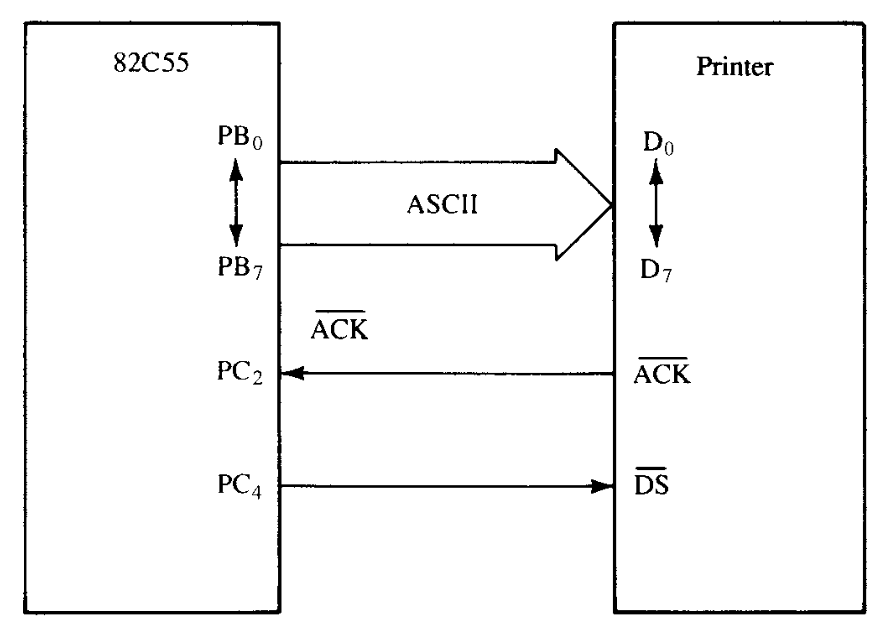
\includegraphics[width = 1.2\textwidth]{./figures/Strobed_Printer.png}
  \caption{Strobed output operation (mode 1) of the 82C55. (a) Internal structure and (b) timing diagram.}
\end{figure}
\begin{itemize}
  \item Port B is connected to a parallel Printer
  \item No signal fto generate the $\overline{DS}$ dignal to the printer.So, PC4 is used with S/W generated $\overline{DS}$.
\end{itemize}

\subsection{Comparison between Mode 1 Strobed Input and Output}

\begin{figure}[h!]
  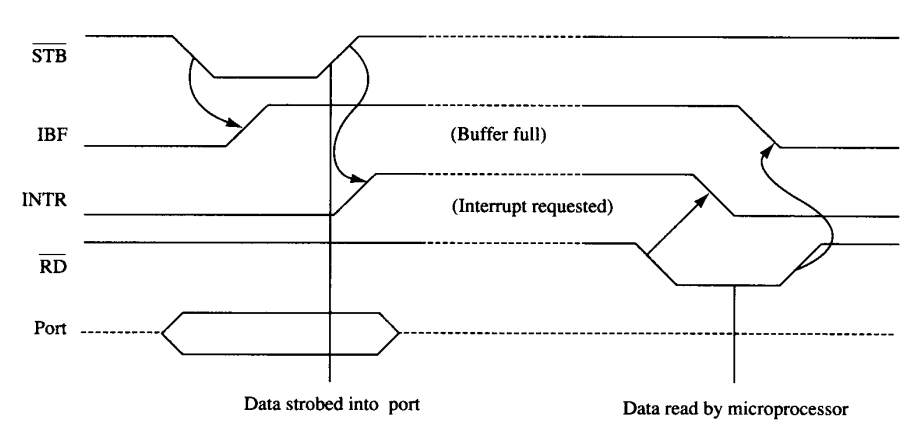
\includegraphics[width = 1.2\textwidth]{./figures/Strobed_I.png}
\end{figure}
\begin{figure}[h!]
  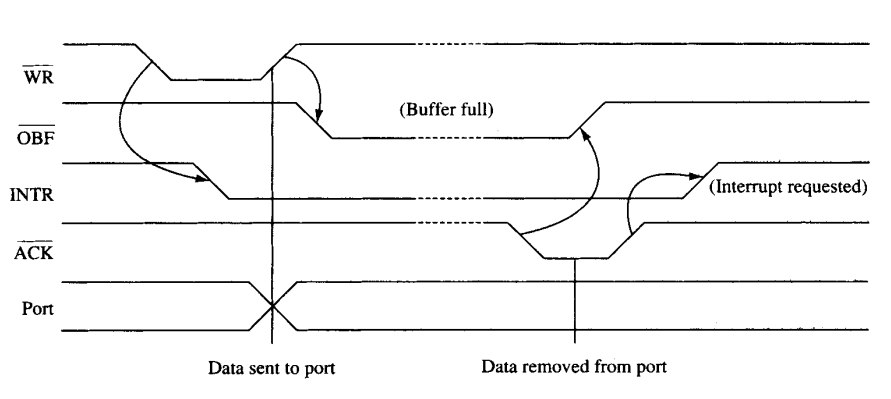
\includegraphics[width = 1.2\textwidth]{./figures/Strobed_O.png}
\end{figure}

\section{Mode 2: Bidirectional Operation}
Group A only; Allows both transmit and receive over the same wires. Useful when interfacing two computers.
\begin{figure}[h!]
  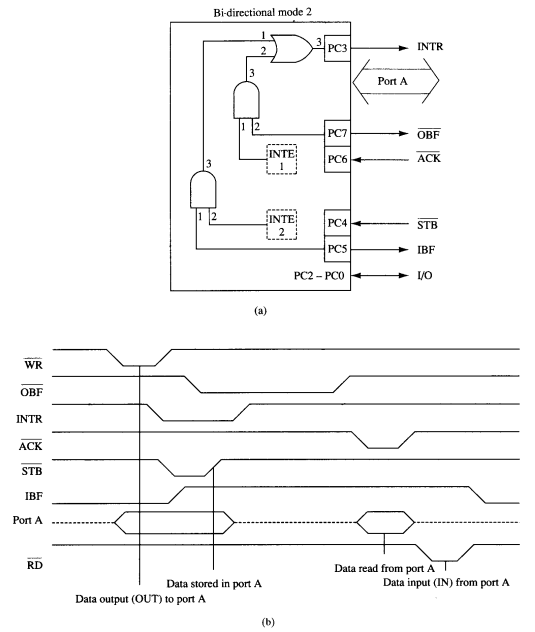
\includegraphics[width = 0.8\textwidth]{./figures/Bi_Directional.png}
  \caption{Mode 2 operation of the 82C55. (a) Internal structure and (b) timing diagram.}
\end{figure}
